% Chapter Template

\chapter{Physical Deployment of Web Applications in Limited Local Space} % Main chapter title

\label{Chapter4} % Change X to a consecutive number; for referencing this chapter elsewhere, use \ref{ChapterX}

\lhead{Chapter 4. \emph{Physical Deployment of Web Applications in Limited Local Space}} % Change X to a consecutive number; this is for the header on each page - perhaps a shortened title

%----------------------------------------------------------------------------------------
%	Deployment
%----------------------------------------------------------------------------------------

One of the earliest problems to come up in developing the screenPerfect sofware has been compromises in how the software is served to users and to artists. The reliance on the internet is difficult, because the internet simply is not always available - it is an unreliable resource that has come to be taken for granted. This is a problem of privacy, partly - anyone can be watched when they're online - but there are also simple installation problems.

WiFi is taken for granted in most institutions, but the fact is that access to these radios must be regulated so that users can be traced, and so that undesirable resources are not accessed. This limitation means that, for security reasons, it is rare that people can share new devices across industrial networks.

There are various circumstances in which one may wish to deploy a web application that do not include areas where a broadband connection to the larger world may be assumed. These areas include many music and art festivals. Any festival directly descended from the Burning Man network, for example, is unlikely to have a reliable connection to the outside world, the point of the events being to form a Temporary Autonomous Zone \cite{taz} to explore broad ideas of art and culture. These zones may nonetheless benefit from art built to take advantage of contemporary smartphones, or contemporary radio technologies, all of which can be operated without a centralized power grid.

There are other challenges to public deployment, such as leaving a valuable production environment out in public, or requiring a technician to look in on specialized equipment. Both of these restrict the venues permitted for public display of work. Also limiting are instances where work should be deployed near people consuming alcohol, which is notoriously bad for electronics.

This chapter addresses my central idea on how to repair the gap between excellent idea for web-based deployment, and the physical reality of gallery spaces with sharply limited resources available for persistent software deployment.

%----------------------------------------------------------------------------------------
%	Problems
%----------------------------------------------------------------------------------------

\section{Problems and Complications in Display}

My method for discovering these issues has been to attempt to display variants of screenPerfect in user testing over the course of a year. We have had exhibits in a van, a tent, and repeated installations at various public bar events. These have been dangerous to electronics. As screenPerfect was developed and extended, and especially after an exhibition at the AGO which resulted in bandwidth throttling, the work began to point in a clear direction: screenPerfect needed to be an arcade box, similar to those used for years in fighting games in bars.

\begin{figure}[h!]
  \caption{psXXYborg van installation}
  \centering
    \includegraphics[width=0.5\textwidth]{psxxyborgvan}
\end{figure}

\begin{figure}[h!]
  \caption{Street Fighter 2 Cabinet}
  \centering
    \includegraphics[width=0.5\textwidth]{streetfighter2}
\end{figure}

Some brainstorming and a very hot summer day resulted in the following scenarios that a reasonable arcade machine would need to address in order to present advanced work to the new, highly exclusive exhibit scenarios.

Here are those design constraints.
\begin{enumerate}
  \item There is never any external data service available.
  In the case of environmental exhibits, or site-specific installation, this is due to location. In the case of formal galleries, it is because bandwidth is not free, or locally reliable. An institution may only have 802.1x limited networks, as in the case of OCADu, or they may simply not have the money to supply thousands of gigabytes of data over the course of an exhibit's lifetime. This must be addressed, as a reliance on the outside means that the art exhibit cannot be reliably collected or maintained.
  \item The exhibit is assumed to be public to anyone, which means that expensive equipment may go missing, or be broken.
  Art exhibits are often displayed in areas with a large audience walking around, and electronics are both delicate and worth money. Electronics purpose-built for exhibition should be easier to install securely in a given context, and harder to sell for parts. 
  \item The environment is assumed to be meterologically hostile - hot or cold, wet or very dry, and to be hosting at least one party, such as an art opening, possibly with music.
  Exhibits outdoors or in new venues, such as Burning Man, are in environments that are terrible for electronics. It is good to put some effort into considering what kinds of devices can survive a rock concert while still displaying the artist's application.
  \item The exhibition is assumed to be supervised by people technically unqualified to maintain a full computer, such as art curators.
  Building computer is a specific trade, as is the curation of artwork. They do not necessarily overlap. A new device should be so easy to use, it runs on being plugged in, and can be trusted to start back up again without trouble when something happens to make it turn off. Any new artwork's support materials should reduce, not increase, the burden of displaying that work, or the work may not be collected or displayed simply due to the massive skills gap between technician and curator.
  \item The emphasis of the work should be on the work's display, rather than on a laptop screen.
  Audiences can be safely assumed to have seen a computer, or a smartphone, perhaps for many hours in their workday. It is therefore preferable to increase the scarcity value and absorption in the work on display by removing the emphasis from a familiar object, such as a laptop, to one with more aura, which could be almost anything but a screen of the standard sort used for brain work in North America. This will improve the value of the work by granting it an air of the exotic, the specific to a single experience.
  \item The collectors of the work are assumed to have extremely limited resources for ruggedized workstations, which are costly.
  Ruggedized workstations, such as would be appropriate for remote environmental display, are costly, because they are designed for \textit{doing} work, rather than \textit{displaying} work. Ruggedization as a design practice stems from both practical considerations, such as bad weather, and a design language derived from military applications. Displaying work using a ruggedized machine brings in both a question of financial access, and an implied language of force which may not be appropriate to the work on display. It is therefore best to separate the specific necessity of waterproofing, dustproofing, impact resistance and heat control from the ideas visible in the typical ruggedized case.
  \item Any data carriage for external connection - wiFi - is assumed to be overloaded by default.
  Art exhibits generally have at least one well-attended party associated with their opening, at which the gallery connection to wiFi is very limited. WiFi is understood to be the "free" access to the internet. For the purposes of this work, it is simply a radio technology. Because the main radio will be overwhelmed by many connections to the outside world, it is best to set up your own network, or captive portal, to serve the information you need served locally, rather than relying on a common carrier for the inside and outside world.
\end{enumerate}

These are all very real constraints that heavily impact the collectibility and display of new media art, most of which is simply difficult to get out the door. We use computers for work and play, but we still separate our lives into periods when we pursue one or the other, and we still have boundaries between our personal and public lives. To use the same machines to display art as we do to \textit{build} the work is to reduce the work from something approachable to any other tab in a computer. New media works especially must be seen within their exhibition context to be understood.

Julia Kristeva addresses this in her essay "Powers of Horror," where she confronts the issue of liminality, and how it holds people's attention

%-----------------------------------
%  Subnod.es, Eyebeam.
%-----------------------------------
\section{Subnod.es and Public Private Space}

This project has a precursor using similar technology built at Eyebeam in New York in 2013. Subnod.es uses a captive portal similar to my own, based on the inexpensive Raspberry Pi framework, to display a chat client to only the local environment. The differences are substantial, although mainly located within the code. Subnod.es relies on an external DNS being made available via the actual subnod.es software, and depends on a different collection of software to serve the portal proper. It is also built such that those library dependencies are inseparable from the main project \cite{subnodes}. 

The chief concern of subnod.es I have not yet mentioned: subnod.es was built as a response to concerns about communications privacy in North America under the NSA. Specifically, the author is concerned that people behave differently when they are watched, a subset of the concerns generally associated with panoptica and totalitarianism. While I have not specifically structured Captive Art Portal to address these concerns, it \textit{has} been built to be largely private. It serves an application to a limited selection of a public space. 

The assumption of the Captive Portal Art Machine is that galleries have limited resources, but that people who go to art galleries almost certainly have access to a smart phone, which is a form of private space. Smart phones are people's own homes, and are built to assume that they will stay with their owners at all times. This means that to install an \textit{app} is to ask a lot of a viewer: specifically, it is to ask someone to bring an application into their private space without getting to sample it first. To contrast, serving that same application on the \textit{broad} internet is to entirely delimit the context the art may be experienced within, which reduces its scarcity value to almost nothing while simultaneously removing the curator's ability to set the context of an exhibition experience. This means that it's unlikely an artist can be compensated in any conventional sense, despite their large audience, and also means that the curation of the exhibit is no different than the "curation" found on Tumblr. Neither of these are fantastic outcomes.

A better outcome is to make a limited public space available in a private context, and this is what we are doing when we ask that people open their phones and look at a website. The Internet is, famously, the new public space. By presenting a web application using public technology within the exclusive context of the gallery - or desert, or forest - we take control again over how our art is presented, and from there, how it can be consumed. A gallery or exhibit space can be set up very specifically for the benefit of an audience in a way that the internet in general cannot be, and web technologies are uniform and affordable in the way that more custom projection design software is not.

This sense of limited private space is key to the code-switching that human communication relies on. We are not the same people in public as we are in private, and we are again different people when we are in different publics, work to the street to school to the gallery. Technology that sensitively addresses these different code contexts seems likely to benefit its authors and its users both.


\section{Materials and Supplies}

This entire build is predicated on a Raspberry Pi running a custom distribution of Debian linux.
\begin{description}
\item [Raspberry Pi] \hfill \\
	The Raspberry Pi is a full linux computer the size of a large credit card. They run Debian linux off of a common SD card.
\item [32Gb SD Card for Raspberry Pi] \hfill \\
	This is where we place the operating system and software for the Pi.
\item [USB wiFi dongle] \hfill \\
	Edimax-based wiFi USB dongle, for serving wiFi hotspot on the Pi.
\item [USB flash memory] \hfill \\
	For transferring or storing complete programs authored on external systems.
\item [Keyboard and Mouse] \hfill \\
	For initial computer setup.
\item [Ethernet Cable] \hfill \\
	Standard cat5 ethernet cable for programming remote.
\item [HDMI TV and cable] \hfill \\
	Used as a monitor for the Raspberry Pi.
\item [Micro USB and power supply] \hfill \\
	Power for the pi.
\item [Mac or PC computer with USB ports, ethernet port, SD Card reader] \hfill \\
	Required for raspberry pi setup.
\end{description}

\section{Background for Linux Commands}

\texttt{sudo} is Linux for Do It Now.

\texttt{apt-get} is an inherited "package manager" from Debian linux. "Dependencies" are the software your software requires to run, Debian uses \texttt{apt-get} to manage them.

Things that follow \texttt{sudo} are commands.

\section{Setting Up Your Raspberry Pi}
\subsection{Windows 7 SD Card setup and first boot}
This section is written for a Windows 7 environment, and is based on the common tutorial at \texttt{http://learn.adafruit.com/adafruit-raspberry-pi-lesson-1-preparing-and-sd-card-for-your-raspberry-pi/}. 

\begin{enumerate}
\item Connect your main computer to the internet.
\item Download the most recent Raspbian distribution image from \texttt{http://www.raspberrypi.org/downloads}.
\item Download Win32DiskImager from the greater internet. This is preferable because it allows you to write image backups to your harddrive.
\item Using Win32DiskImager, write your Raspbian distro to your SD card on your main computer.
\item Eject the microSD card and stick it into your RasPi.
\item Plug in your keyboard, and plug a mouse into your keyboard.
\item Plug in your HDMI cable and monitor. Turn them on.
\item Plug in the MicroUSB cable for power to your RasPi.
\end{enumerate}

\subsection{Configuring Raspbian}

Once the RasPi is turning on, it needs to be set up to include all of its software. Turn the Pi on, and wait until the blue configuration screen comes up.

\begin{figure}[h!]
  \caption{Early RasPi Configuration Screen}
  \centering
    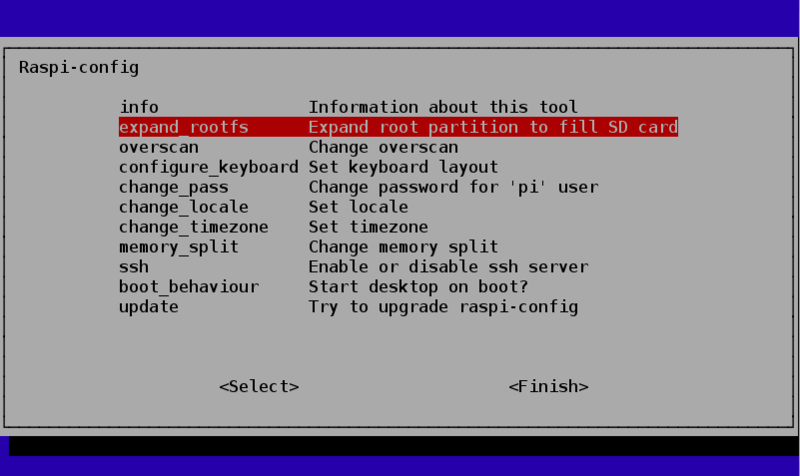
\includegraphics[width=0.5\textwidth]{raspi-config_expand_1.png}
\end{figure}

\begin{enumerate}
\item \textit{expand\_rootfs} Expand the boot system so that you will not run out of onboard memory for software.
\item \textit{memory\_split} Reduce the GPU to minimum, because we will be using the raspi as a headless server from the command line.
\item \textit{change\_pass} Change the password so that your raspi will be less easy to hack.
\item \textit{ssh} Enable SSH so that the pi will be accessible from an external computer.
\end{enumerate}

When done, select \texttt{finish} to exit. 

Type \texttt{sudo reboot} to restart the raspi.

\section{Software Setup for External WiFi Access}

A wiFi antennae can be used for one purpose at a time: it can either be used to access the external internet, for acquiring software to install into the raspi, or it can be used for serving a hotspot. It cannot do both at the same time. To load the pi up requires external access, so we will be loading that first. You must configure your wiFi before plugging in your wiFi antenna.

In Linux, nothing will warn you if you mistype a folder name, say, adding an "s" to "network" to make it "networks." If you would like to confirm your folder name is correct, try typing "ls /etc/" to list the contents of that directory. Network is a default folder, and Interfaces is already present at first boot, so you can make sure your things are all there before you really get started.

The way to tell you have done something wrong is if you type the below command and an empty new file opens. You are editing a file here, not creating one.

At your console prompt, type the following: 
\begin{lstlisting}
sudo nano /etc/network/interfaces
\end{lstlisting}

This opens a text editor. Enter the following into it.

\begin{lstlisting}
auto lo

iface lo inet loopback
iface eth0 inet dhcp

allow-hotplug wlan0
auto wlan0

iface wlan0 inet dhcp
wpa-ssid "network name, commonly called an ssid, goes here"
wpa-psk "password"
\end{lstlisting}

Then type CTRL-X and Y to save your file.

\begin{lstlisting}
sudo halt
\end{lstlisting}

Plug in your wifi antennae, pull your raspi's power cable, and plug it back in. This should make the raspi's antennae turn blue as it turns on. This little blue LED will frequently be the only way to tell something is going correctly or incorrectly, so it is an excellent tell that your machine is running. 

\begin{figure}[h!]
  \caption{Raspberry Pi with functioning wiFi antenna}
  \centering
    \includegraphics[width=0.5\textwidth]{raspi_with_wiFi_on}
\end{figure}

If all went well, you've now connected to your own supply of wireless internet. This will not work if you are using an 802.1x network, such as those within OCADu. On your own home network, however, type:

\begin{lstlisting}
sudo apt-get upgrade; sudo apt-get update
\end{lstlisting}

This will upgrade your rasppi to whatever the latest agreed-upon package lists are, then update those packages to their most recent approved version.

\section{Installing Node.JS}
\subsection{Why Node?}
I've chosen to install Node because it is the software framework I selected to run the new game engine built in Part 1 of this thesis. Node is a new framework designed to get Javascript running on a server. There are advantages and disadvantages to this approach. The advantages are that JavaScript is a beautiful, minimal language that is relatively easy to learn. The disadvantages are that there is a heavy public bias against JS due to its years as a client-only language designed to manipulate what are known as Document Object Model (DOM) elements in-browser.

The brilliance of Node is that it replaces the need for a specific input-output window, replacing that definition requirement with any internet browser. Node, backed by Google's V8 engine, currently works best on Chrome, but it can interact with any browser.

Node is therefore easy to use, and easy to program for from the perspective of a mainly web based development chain. 

\subsection{Installation Instructions for Node.JS}
Create a directory for Node to live in by typing the following at prompt.
\begin{lstlisting}
sudo mkdir /opt/node
\end{lstlisting}

Acquire the node "tarball" - compressed framework files - via the internet.

\begin{lstlisting}
wget http://nodejs.org/dist/v0.10.2/node-v0.10.2-linux-arm-pi.tar.gz
\end{lstlisting}

Unzip (desticky from tarball) it:
\begin{lstlisting}
tar xvzf node-v0.10.2-linux-arm-pi.tar.gz
\end{lstlisting}

Copy the contents of the newly unzipped folder and paste them to your new directory. This leaves a copy of the tar and a copy of the unzipped tar at their original locations. You can probably remove them using sudo rm when you're sure everything is where it should be.

\begin{lstlisting}
sudo cp -r node-v0.10.2-linux-arm-pi/* /opt/node
\end{lstlisting}

Edit - or create - a .bash_profile file, which is a type of script that runs when you turn on the pi. In this case, it runs and tells Node that it exists on your computer, so that typing node runthisprogram will do something. What is a .bash_profile?

From your root directory, to open a new nano text file:
\begin{lstlisting}
sudo nano .bash_profile 
\end{lstlisting}

Then add the following and save it to your new .bash_profile file...

\begin{lstlisting}
PATH=$PATH:/opt/node/bin 
export PATH
\end{lstlisting}

Control-X, Y to save it.

Node lives in the \texttt{/opt/node} directory you created above. This adds the commands "node" and "npm" to what are called "environment variables." If you are curious, and god knows you must be to play with a raspi, you can type \texttt{ls /opt/node/bin} and see the little programs sitting there in their bin.

\section{Testing Node}
Node will need to be able to fetch its own packages separately from the raspi from the internet in order to run some of the monitoring software I've chosen to use. Particularly, you will need the \texttt{forever} package.

\subsection{Selecting Monitoring Software}
\texttt{forever} has ultimately been the software I've decided on to monitor and run screenPerfect, because it is a node-native package that keeps things running even when they crash. There are other software packages used for broader deployment, such as Monit, which installs to your Debian parcel rather than to Node. Monit typically runs with what is called an HTTP Proxy, which can be written directly in Node or installed independently. In a full deployment build, Monit and HAProxy would be preferable to Node alone, because this follows the best practice of separating out different programming elements from one another in production. Monit and HAProxy can also deploy applications above and beyond Node itself, which is preferable for things written in Python, for example. 

For this example, though, \texttt{forever} works well. It provides monitoring to tell us what the application is doing, and automatically restarts node applications when they crash. Were I deploying this such that it could keep an eye on the internet, which I am not, I would also include \texttt{nodemon}, as is recommended by the Subnod.es project. \texttt{nodemon} monitors your development code and pushes changes from a central server to your deployment automatically.

That is outside the scope of this paper at present. 

\subsection{Installation of Node Modules}
To install a node package - or "module" - you type 

\begin{lstlisting}
npm install PACKAGENAME
\end{lstlisting}

To install one globally, type
\begin{lstlisting}
npm install PACKAGENAME -g
\end{lstlisting}


To absolutely force install:
\begin{lstlisting}
sudo su
PATH=/opt/node/bin/:$PATH
npm install PACKAGENAME -g
exit
\end{lstlisting}

To install \texttt{forever} and \texttt{nodemon}
\begin{lstlisting}
npm install forever -g
npm install nodemon -g
\end{lstlisting}

To run \texttt{forever} and \texttt{nodemon} together....
\begin{lstlisting}
forever start /usr/local/bin/nodemon /path/to/YOURAPP.js
\end{lstlisting}

\subsection{Troubleshooting NPM installations}
When I tried to install \texttt{forever} the first five times, it timed out, gave me a 404 error repeatedly, and declared I had insufficient permissions to do a global install. This is where computer science faith, confidence, and patience come in. When the install did not work for half an hour, I took a break, came back, and discovered that it installed the next day.

This process is heavily dependent on a massive network of computers and other people. In development, it is quite likely things beyond one's own control are going to go wrong. Going for a break will help you keep patient.

\section{SSH via Direct Ethernet Connection and WiFi Internet Access}
Eventually, you will need both of the powered USB slots on the raspi for a USB key and for your wiFi. In addition, the raspi doesn't have the power to drive a monitor and consistently serve wiFi out of its USB ports. To get around this, it is most convenient to be able to SSH in to your device. Although it appears to be best practice to use the wpa_supplicant file to store how you wish your raspi to connect to the internet, I have had limited success with it, likely because I am not configuring a static IP for my raspi properly.

My \texttt{/etc/network/interfaces} file looks like this:
\begin{lstlisting}
auto lo
iface lo inet loopback

auto eth0
iface eth0 inet static
address [MY MAIN TERMINAL'S ETHERNET IP PLUS ONE]

auto wlan0
allow-hotplug wlan0
iface wlan0 inet dhcp
     wpa-ssid "network name here"
     wpa-psk "dubiously secure password"
\end{lstlisting}
 

\begin{lstlisting}
sudo nano /etc/default/ifplugd

### MANY TALK, HOW COMMENT, SUCH WARNING ###
INTERFACES="eth0"
HOTPLUG_INTERFACES="eth0"
ARGS="-q -f -u0 -d10 -w -I"

SUSPEND_ACTION="stop"
\end{lstlisting}

This is an edit of the existing bits, and I can't tell if it will break everything long-term.
Here is what your startup script should read. This ensures that your wiFi antenna turns on, which is likely not something it was doing when you plugged in your ethernet directly.

\begin{lstlisting}
sudo nano /etc/rc.local
#!/bin/sh -e

# Print the IP address
_IP=$(hostname -I) || true
if [ "$_IP" ]; then
  printf "My IP address is %s\n" "$_IP"
fi

# Disable the ifplugd eth0
sudo ifplugd eth0 --kill
sudo ifup wlan0

exit 0
\end{lstlisting}

CTRL-X and Y to save, then \textttt{sudo reboot} open a terminal on your main laptop. On your laptop, at the prompt, enter:
\begin{lstlisting}
ssh pi@[the static ip address you entered under eth0 static above]
\end{lstlisting}

Your \texttt{pi@[static ip]} should appear in your terminal window, which means you can now talk to raspi.
Per usual, to ensure your wifi is still working properly, try a \texttt{sudo apt-get update} or \texttt{ping google.com}, both should return you data.

\section{Backing Up Your RasPi}

Now that everything has been configured for the first steps, type \texttt{sudo halt}, and when your raspi turns off, remove the SD card from it. Place the SD card back in your main computer and reboot Win32DiskImager.

Create a new file folder somewhere within your Documents folder. I called mine Raspberry Pi Backups.

In the Write From section of the application, select your SD card, which is probably called boot. In the Write To section, select your new folder. 

Write a copy of the kernel image from the boot card to the new backup directory. Then safely eject your SD Card and re-insert it in the RasPi. It is best practice to form these occasional backups as you proceed through set up. Many of these steps can cause your raspi distro to break badly. A backup will save a great deal of time when the inevitable happens.

\section{Mount Your USB Flash Memory Stick To Your RasPi}

\subsection{Configuring Your Mount Drive}
This bears some thinking about, because the \texttt{/media/} folder is for media, and you are instead choosing to run a program off of the drive. Subnod.es suggests making it your \texttt{www} drive, for world wide web. I picked \texttt{/mnt/}.

Find your USB memory by listing the the things plugged into dev:
\begin{lstlisting}
sudo ls /dev/sd*
\end{lstlisting}

If you've been following along, yours is almost certainly named "/dev/sda1".

So make a directory for it to be addressed at:
\begin{lstlisting}
sudo mkdir /mnt/USBSTICKNAME;
\end{lstlisting}

Then mount it to that directory
\begin{lstlisting}
sudo mount -t vfat -o uid=pi,gid=pi /dev/sda1 /mnt/USBSTICKNAME/
sudo reboot
\end{lstlisting}

Rebooting will restart the raspi but also close your SSH session. Watch the lights on the raspi board until they're stable again, about two minutes, then:
\begin{lstlisting}
ssh pi@[static ip]
\end{lstlisting}

Oh look. Your USB drive does not automatically mount at boot. Problem.

\subsection{How to Boot Mount External Memory}

Find out the actual name of your external memory card:
\begin{lstlisting}
ls -l /dev/disk/by-uuid
\end{lstlisting}

Write down the UUID of your USB stick.

This is the most manual way to run this operation, and there is software that handles automatic drive mounting. It is called \texttt{usbmount} and was discarded during this process because it ended up being more convenient to rely on my Node application being loaded directly onto the SD card, rather than from boot.

\begin{lstlisting}
sudo chmod 775 /mnt/USBSTICKNAME
sudo sp /etc/fstab /etc/fstab.bak
sudo nano /etc/fstab
\end{lstlisting}

Add the following to \texttt{/etct/fstab}
\begin{lstlisting}
UUID=YOURUUID /mnt/USBSTICKNAME vfat rw,defaults 0 0
\end{lstlisting}

CTRL-X, Y to save, then
\begin{lstlisting}
sudo reboot
ls /mnt/USBSTICKNAME
\end{lstlisting}

This command should display the contents of your USB key when you go looking for it.

At this point, I have taken a copy of my Node application and moved it to the SD card in a separate directory. Although I have optimistically tried to make this a headless - no keyboard or monitor - box, realistically, lots can go wrong with the SSHing process. You will probably eventually want a keyboard, and it is _much_ easier to store your access point as a single image per card, much like any other video game.

To store your games locally, rather than in the USB stick:
\begin{lstlisting}
sudo cp -r /mnt/USBSTICKNAME /home/pi/YOURDIRECTORYNAME
\end{lstlisting}

\section{Set Up a wiFi Hotspot}
To get started, you will need some more software.

\begin{lstlisting}
sudo apt-get install hostapd dnsmasq
\end{lstlisting}

When everything is done installing, you will be converting your \texttt{/etc/network/interfaces} file to serve a hotspot, rather than connect to the internet. 

Here is what my final \texttt{/etc/network/interfaces} file looks like:

\begin{lstlisting}
auto lo
iface lo inet loopback

auto eth0
iface eth0 inet static
     address 169.254.222.xx #xx is a stand-in for an actual address, not included.

allow hotplug wlan0

## wlan internet connect settings are commented out for easy swap.
#auto wlan0
#iface wlan0 inet dhcp
#     wpa-ssid "network name"
#     wpa-psk "network password"

iface wlan0 inet static
     address 192.168.42.1 #42 is a joke about Douglas Adams, in honour of my thesis advisor.
     netmask 255.255.255.0

\end{lstlisting}

\section{Configuring HostAPD}
\textt{hostapd} is the software that provides the access point using your raspi. It can be tricky, and in order to make it work, it needs to be compiled for one's specific model of wiFi antennae. For the purposes of this paper, we are using an antenna sold and supported by Adafruit. The appropriate compile of the hostapd software is included in the supplementary files to this paper, but can also be found at http://www.adafruit.com/downloads/adafruit_hostapd.zip.

To install a valid copy of hostapd:
\begin{lstlisting}
wget http://www.adafruit.com/downloads/adafruit_hostapd.zip 
unzip adafruit_hostapd.zip 
sudo mv /usr/sbin/hostapd /usr/sbin/hostapd.ORIG 
sudo mv hostapd /usr/sbin
sudo chmod 755 /usr/sbin/hostapd
\end{lstlisting}
 
Now set up a daemon - a piece of automatic system software - to run the hostapd configuration file on boot.
\begin{lstlisting}
sudo nano /etc/default/hostapd
\end{lstlisting}
Uncomment (remove the hash mark in front of) \texttt{#DAEMON_CONF=""} and replace that line with \texttt{DAEMON_CONF="/etc/hostapd/hostapd.conf}.
Then type CTRL-X and Y to save your file.

My hostapd file is listed below.

\begin{lstlisting}
sudo nano /etc/hostapd/hostapd.conf

interface=wlan0
driver=rtl871xdrv
ssid=piebox
hw_mode=g
channel=6
macaddr_acl=0
auth_algs=1
ignore_broadcast_ssid=0
wpa=2
wpa_passphrase=berrybox
wpa_key_mgmt=WPA-PSK
wpa_pairwise=TKIP
rsn_pairwise=CCMP

\end{lstlisting}


\section{Configuring DNS access via \texttt{dnsmasq}}

Configuring \textt{dnsmasq} is straightforward. The installation package comes with an extensive config file, which lives at \texttt{/etc/dnsmasq.conf}, and includes all of the options necessary to turn on a DNS routing service.

To configure your dnsmasq installation, enter \texttt{sudo nano /etc/dnsmasq.conf} and then add the following lines to the top of the configuration file. The configuration file contains all these values commented out already, and may be worth a separate read.

\begin{lstlisting}
interface=wlan0
dhcp-range=192.168.42.2, 192.168.42.50,255.255.255.0,12h
address=/#/192.168.42.1 #redirect all DNS requests to 192.168.42.1
server=/screenperfect/192.168.42.1#3003
address=/apple.com/0.0.0.0
\end{lstlisting}

What the above does is tell the raspi to listen on the wlan0 interface, to the dhcp range between 192.168.42.2 and 42.50, for twelve hours per time a client connects to the wiFi point. In addition, the portal is supposed to redirect all DNS requests - things like "google.com" - to the Pi's main address, which is - as we can see in \texttt{/etc/network/interfaces} - 192.168.42.1, and from there to the port 3003, on which my particular Node application listens.

In addition, the portal serves a spoof address to apple.com, which helps us to pop up the appropriate page on the captive portal when it is turned on. 

At this point, reboot the raspi by typing \texttt{sudo reboot} and everything should come up properly and turn on appropriately.

\subsection{IP Addresses}
The trickiest part of this particular operation is the various IP addresses. IP addresses are raw internet magic. They are how we phone the internet, and how we talk to things once all the radios are tuned in, and they are admirable. From Wikipedia....

\section{Setting Up init.d to Run \texttt{forever} as a Boot Script}